%%%%%%%%%%%%%%%%%%%%%%%%%%%%%%%%%%%%%%%%%%%%%%%%%%%%%%%%%%%%%%%%%%%%%%%%
% Plantilla TFG/TFM
% Escuela Politécnica Superior de la Universidad de Alicante
% Realizado por: Jose Manuel Requena Plens
% Contacto: info@jmrplens.com / Telegram:@jmrplens
%%%%%%%%%%%%%%%%%%%%%%%%%%%%%%%%%%%%%%%%%%%%%%%%%%%%%%%%%%%%%%%%%%%%%%%%

\chapter{State of the Art}
\label{marcoteorico}

In the second chapter of this thesis, we will examine the \textit{state-of-the-art} approaches and provide the theoretical background relevant to the key components of this research. The discussion will follow a structured progression, gradually building a conceptual foundation for the proposed system.

We will begin by exploring how \textbf{action and motion can be captured from video data using deep learning techniques}, focusing on the development of algorithms that interpret movement frame by frame. This section will highlight the evolution of video-based motion analysis, starting with applications involving \textbf{human subjects}, which have served as the primary benchmark in the field due to the early availability of annotated datasets and the demand for human activity recognition in areas such as surveillance, healthcare, and human-computer interaction.

From there, we will transition to the \textbf{application of motion capture technologies in animals}, a direction that has gained momentum primarily since the 2010s with the rise of non-invasive video analysis and advancements in computer vision. Finally, the focus will narrow to \textbf{birds}, which represent the central subject of this thesis. We will review existing work on bird detection and tracking, discuss the unique challenges of avian motion analysis, and present how recent methods are beginning to bridge the gap between human-centered models and their adaptation to the animal domain.



\section{CNNs and Transformers for Video Analysis}

In the context of bird behavior analysis, both Convolutional Neural Networks (CNNs) and Vision Transformers (ViTs) — along with their hybrid variants (Hybrid Vision Transformers, or HVTs) — offer promising architectures. CNNs are effective at capturing local spatial patterns and are well-suited for recognizing short, localized actions. ViTs, leveraging self-attention, excel at modeling long-range dependencies, making them useful for understanding complex behavioral sequences.

Hybrid models aim to combine the strengths of both approaches by integrating convolutional operations into transformer architectures. This enables better performance in tasks that require both local feature extraction and global context modeling.

These architectures can also serve as strong alternatives for building generative models — for example, in reconstructing or simulating bird behavior from video data.

\subsection{The Inductive Bias of Convolutional Neural Networks (CNNs)}
For many years, CNNs have been the cornerstone of state-of-the-art results in nearly all computer vision tasks. Their success is rooted in a strong and highly effective \textbf{inductive bias} for processing images. The core operation of a CNN is the convolution, where a small, learnable filter (or kernel) slides across the input image, computing dot products at each position. This design inherently possesses two key properties:

\begin{itemize}
    \item \textbf{Locality:} The convolutional operation processes only a small, local neighborhood of pixels at a time. This is based on the assumption that pixels that are spatially close are semantically related, which is a powerful and efficient prior for image data.
    \item \textbf{Translation Equivariance:} Because the same filter is applied across all spatial locations, a CNN can recognize a pattern regardless of where it appears in the image. This weight-sharing mechanism makes CNNs remarkably parameter-efficient.
\end{itemize}

These properties allow CNNs to build a hierarchical representation of an image, learning simple features like edges and textures in early layers and composing them into more complex object parts in deeper layers. However, this strength in local processing is also a limitation. The receptive field of any given neuron is spatially constrained, making it difficult for standard CNNs to model explicit, long-range dependencies between distant parts of an image without a very deep hierarchy of downsampling operations.

\begin{figure}[H]
    \centering
    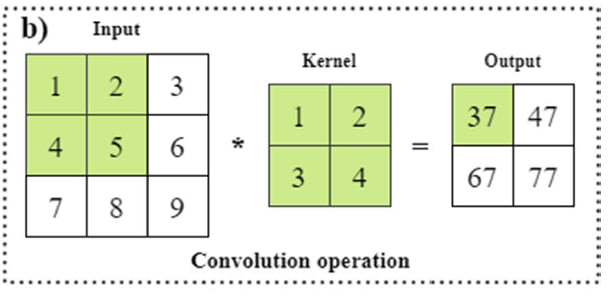
\includegraphics[width=0.8\textwidth]{archivos/figuras/convolution.jpg} 
    \caption{The convolution operation, illustrating the local processing nature of CNNs.}
    \label{fig:convolution}
\end{figure}

\subsection{Vision Transformers (ViTs) and the Global Context}
Inspired by the immense success of Transformers in Natural Language Processing (NLP), the Vision Transformer (ViT) was proposed as an alternative architecture for vision tasks. ViTs discard the idea of convolutions entirely and instead rely on the \textbf{self-attention mechanism}. The standard ViT pipeline operates as follows:

\begin{enumerate}
    \item \textbf{Image Patching:} The input image is divided into a grid of fixed-size, non-overlapping patches.
    \item \textbf{Linear Projection:} Each patch is flattened into a 1D vector and linearly projected into a vector space, creating a sequence of "patch embeddings."
    \item \textbf{Positional Encoding:} Since the self-attention mechanism is permutation-invariant (it does not inherently understand the order or position of elements), learnable positional embeddings are added to the patch embeddings to retain spatial information.
    \item \textbf{Transformer Encoder:} This sequence of vectors is fed into a Transformer encoder, composed of multiple layers. Each layer's core components are a Multi-Head Self-Attention (MSA) module and a feed-forward Multi-Layer Perceptron (MLP).
\end{enumerate}

The MSA mechanism is the key innovation. It calculates the relationships between all pairs of patches in the sequence simultaneously, producing an attention map that weighs the importance of every patch relative to every other patch. This allows ViTs to model the \textbf{global context} of an image from the very first layer. However, this power comes at a cost. ViTs lack the built-in inductive biases of CNNs, making them less sample-efficient. They often require training on massive datasets (e.g., ImageNet-21k, JFT-300M) to learn fundamental visual concepts that CNNs acquire naturally.

\begin{figure}[H]
    \centering
    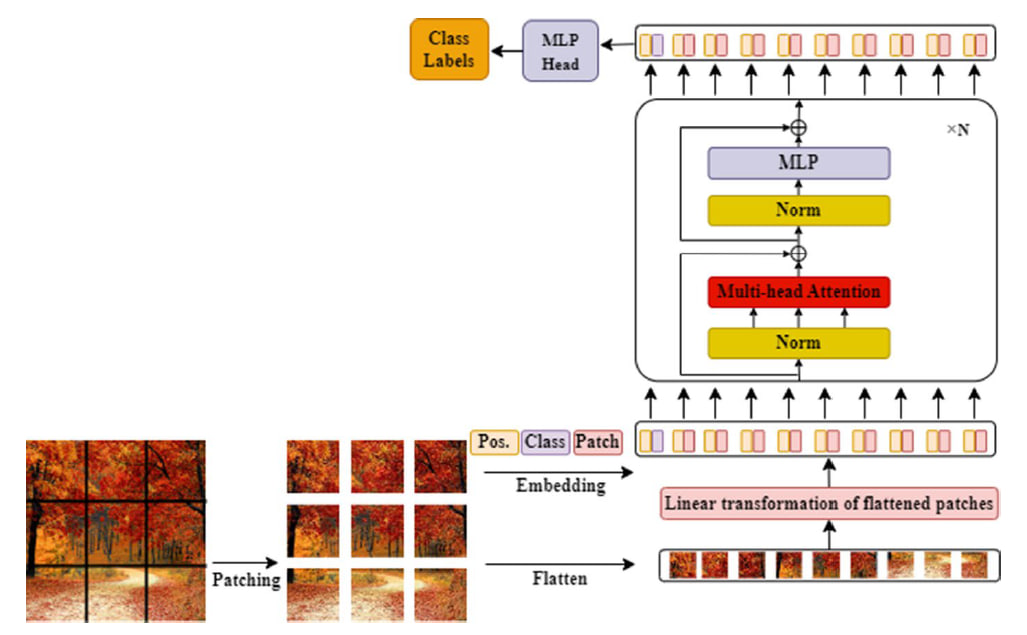
\includegraphics[width=0.8\textwidth]{archivos/figuras/ViT.jpg} 
    \caption{The detailed architecture of a standard Vision Transformer (ViT).}
    \label{fig:vit_arch}
\end{figure}

\subsection{The Synthesis: Hybrid Vision Transformers (HVTs)}
The complementary nature of CNNs and ViTs—one excelling at local, hierarchical feature extraction and the other at global context modeling—has naturally led to the development of \textbf{Hybrid Vision Transformers (HVTs)}. These architectures aim to create a synergy between the two, injecting the beneficial inductive biases of convolutions into the powerful self-attention framework. The goal is to build models that are both highly performant and data-efficient. The survey by Khan et al. provides a comprehensive taxonomy of how this integration can be achieved.

\begin{figure}[H]
    \centering
    % You must have the image file in your project directory
    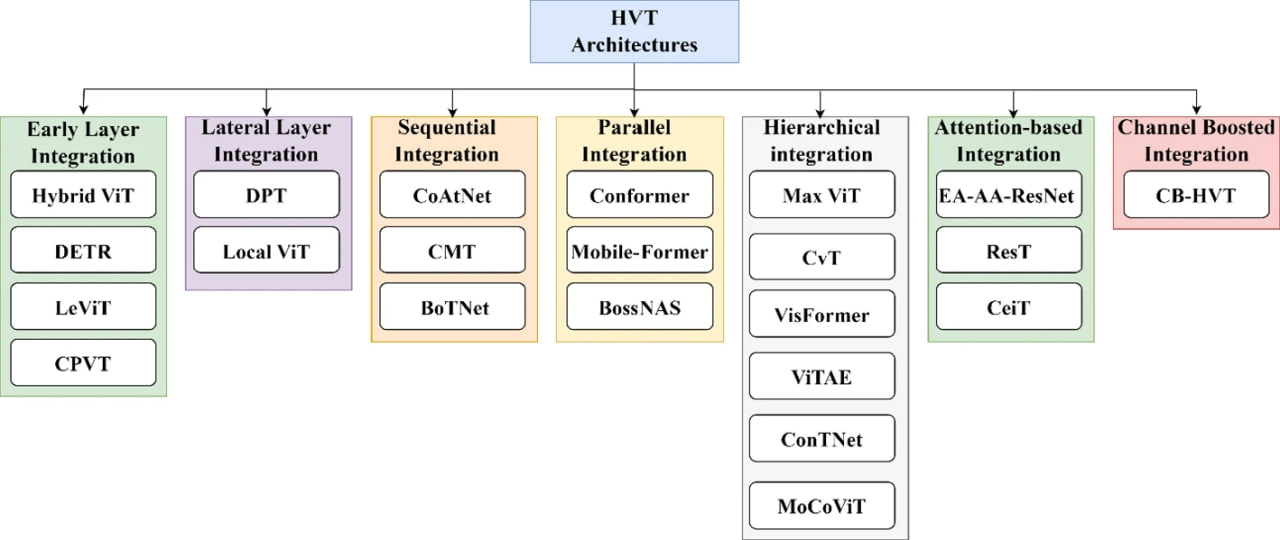
\includegraphics[width=0.8\textwidth]{archivos/figuras/hvt.jpg} 
    \caption{A taxonomy of Hybrid Vision Transformer architectures, classifying models based on their integration strategy.}
    \label{fig:hvt_taxonomy}
\end{figure}

\subsection{CNN-Transformer Integration Architectures}

Various strategies have been proposed to combine Convolutional Neural Networks (CNNs) with Transformer architectures, aiming to leverage the strengths of both. These hybrid designs can be broadly categorized into four integration patterns:

\begin{enumerate}
    \item \textbf{Early-layer Integration:} A CNN backbone processes the input image into rich feature maps that encode local patterns and spatial hierarchies. These maps are then tokenized and passed to a Transformer encoder. This allows the transformer to operate on semantically meaningful features from the beginning. Examples include \textbf{DETR} and \textbf{LeViT}.

    \item \textbf{Sequential Integration:} Convolutional and transformer blocks are stacked in series. Typically, the model begins with convolutional layers, followed by hybrid blocks (e.g., CMT) that incorporate both local feature extraction and lightweight attention. This enables progressive refinement of both local and global features.

    \begin{figure}[H]
        \centering
        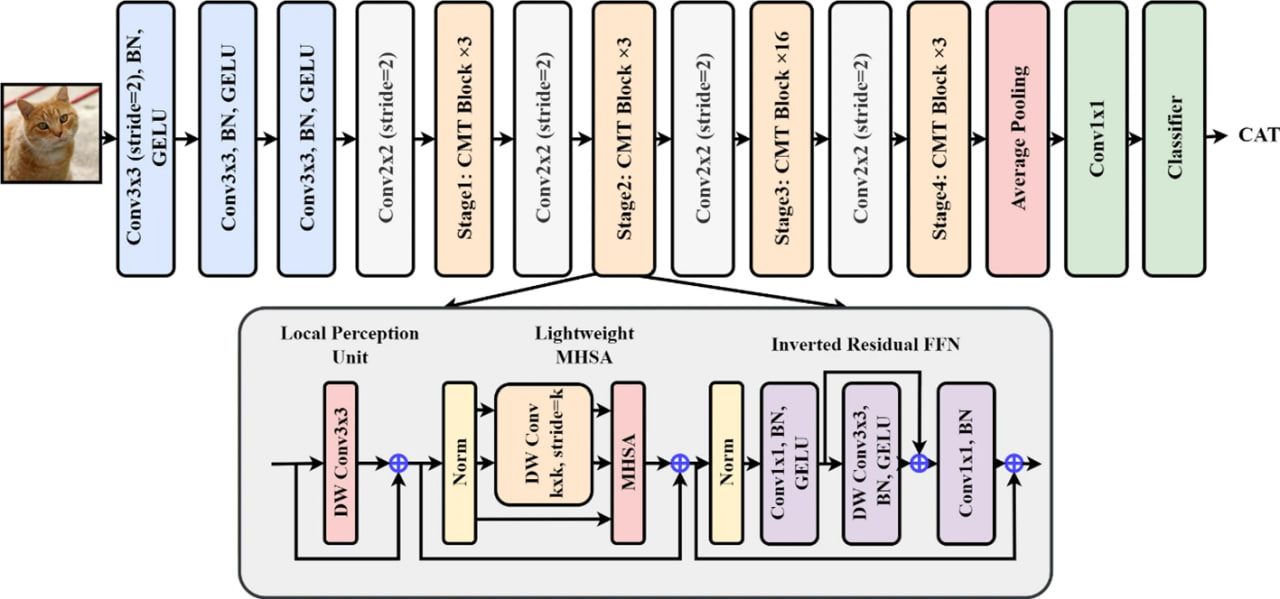
\includegraphics[width=0.8\textwidth]{archivos/figuras/cmt.jpg}
        \caption{An example of a sequential integration architecture: CMT.}
        \label{fig:cmt_arch}
    \end{figure}

    \item \textbf{Parallel Integration:} CNN and Transformer branches operate concurrently, each focusing on local and global features respectively. Information is exchanged and fused at multiple stages to produce a joint representation. A prominent example is the \textbf{Conformer} architecture.

    \item \textbf{Hierarchical Integration:} Inspired by CNN pyramidal structures (e.g., ResNet), these models process features at multiple scales, combining convolution and attention within each stage. Patch merging or downsampling reduces resolution while increasing channel depth. \textbf{Swin Transformer} and \textbf{MaxViT} are leading models in this category.
\end{enumerate}

These integration strategies form the foundation of Hybrid Vision Transformers (HVTs), which are particularly relevant for tasks involving structured, multi-scale, or temporal data—such as recognizing complex bird behaviors from video.


\section{Overview of Deep Learning for Video Scene Analysis}

The analysis of bird behavior in video data shares common challenges with general video scene understanding. Early approaches relied on handcrafted features such as SIFT, HOG, or optical flow, which were manually designed and then passed to separate classifiers like SVMs. Although these methods could be effective in constrained environments, they often lacked robustness and scalability.

The advent of deep learning shifted the field toward end-to-end models that learn spatio-temporal features directly from raw video frames. This is particularly important for capturing subtle and temporally extended patterns typical of animal behavior. Modern architectures — including encoder-decoder models, attention mechanisms, and transformer-based networks — provide powerful tools for recognizing and modeling such behavior.

Core deep learning components used in video analysis include Convolutional Neural Networks (CNNs) for spatial feature extraction and Recurrent Neural Networks (RNNs) or Transformers for modeling temporal dynamics. These components are often combined to capture both the fine-grained motion and the long-term structure present in behavioral sequences.

\subsection{Convolutional Neural Networks (CNNs) for Spatial Understanding}
CNNs are the workhorse of modern computer vision. As detailed in Section 2.1.1 of the survey, their architecture is specifically designed to process grid-like data such as images. By using learnable filters and shared weights, they efficiently capture spatial patterns. In the context of video analysis, a CNN is typically applied on a frame-by-frame basis to act as a powerful feature extractor. The network processes each frame to identify objects, scenes, and body parts, thus encoding the \textbf{spatial} information of the video. The output for each frame is a compact feature vector that represents its content.

\begin{figure}[H]
    \centering
    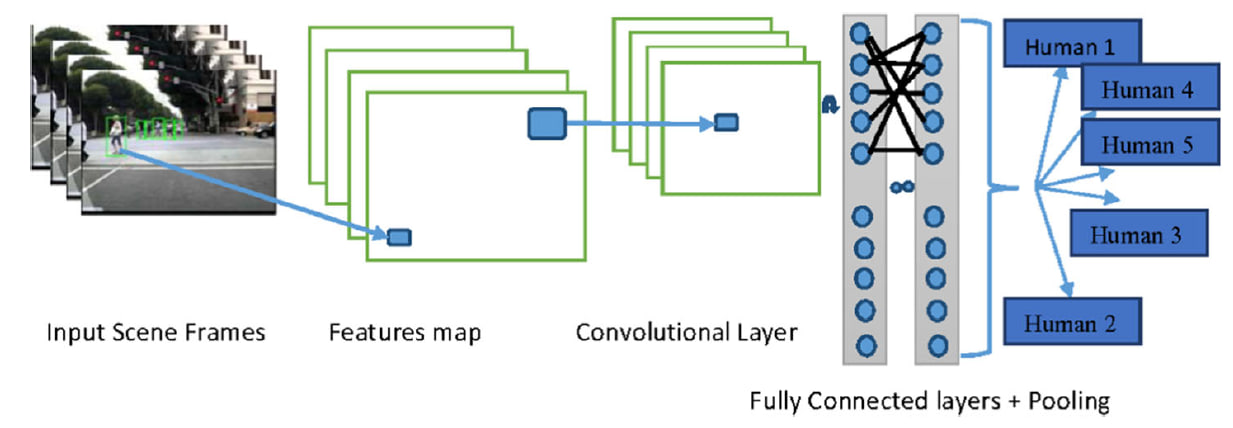
\includegraphics[width=0.8\textwidth]{archivos/figuras/CNN.jpg} 
    \caption{An illustration of a human object recognition system using a CNN.}
    \label{fig:cnn_recognition}
\end{figure}

\subsection{Recurrent Neural Networks (RNNs) for Temporal Dynamics}
While CNNs excel at understanding static frames, they inherently lack a mechanism to model the \textbf{temporal} dimension of video. Actions and events are, by definition, sequences that unfold over time. Recurrent Neural Networks (RNNs) are specifically designed to handle such sequential data. As described in Section 2.1.2, RNNs possess a feedback loop, allowing them to maintain an internal state or "memory" of past information. This enables them to learn temporal patterns from a sequence of inputs. For video analysis, the Long Short-Term Memory (LSTM) variant of RNNs is particularly popular due to its ability to capture long-range dependencies.

\subsection{Hybrid CNN-RNN Models: The Standard for Activity Recognition}
The most effective and widely adopted approach for video-based activity recognition is to combine the strengths of CNNs and RNNs into a hybrid architecture. In this model:
\begin{enumerate}
    \item The \textbf{CNN} acts as a per-frame feature extractor. It processes each frame of the video independently and outputs a sequence of feature vectors.
    \item The \textbf{RNN (LSTM)} takes this sequence of feature vectors as its input and models the temporal evolution between them to recognize the underlying activity.
\end{enumerate}
This two-stage process allows the model to learn both "what" is in the scene (via the CNN) and "how" it is changing over time (via the RNN), which is essential for robust action recognition.

\begin{figure}[H]
    \centering
    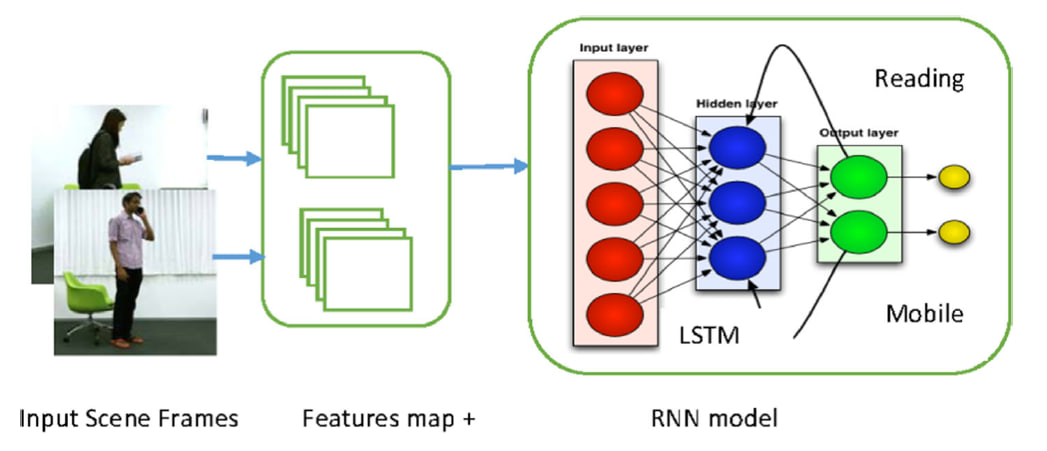
\includegraphics[width=0.8\textwidth]{archivos/figuras/recognition.jpg} 
    \caption{The architecture of a hybrid CNN-RNN system for human activity recognition.}
    \label{fig:cnn_rnn_activity}
\end{figure}

\section{A Taxonomy of Video Analysis Applications}

Deep learning models are not monolithic; they are adapted and combined to solve a variety of specific tasks within the broader field of video scene analysis. The survey provides an application-oriented taxonomy, mapping different problems to the deep learning methods used to solve them. This demonstrates the modularity and versatility of the core architectures.

\begin{figure}[H]
    \centering
    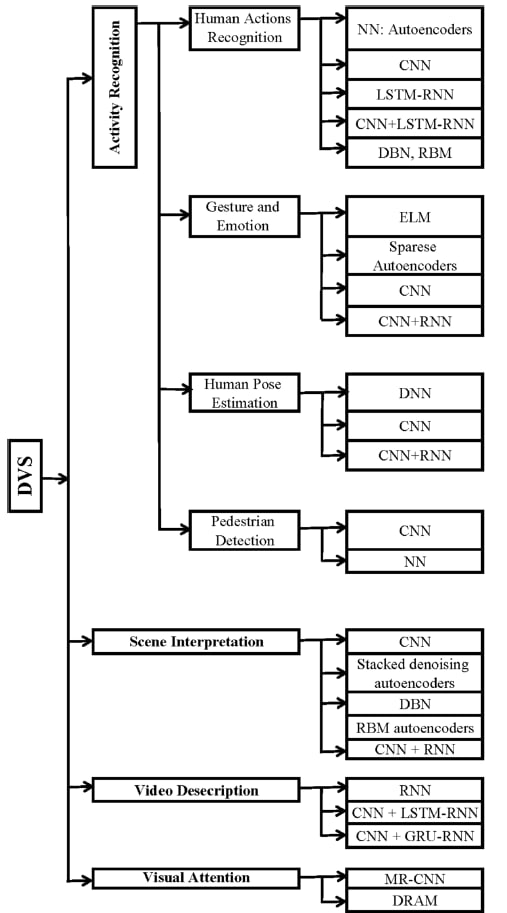
\includegraphics[width=0.8\textwidth]{archivos/figuras/dvs.jpg} 
    \caption{An application-based taxonomy of deep learning methods used in Deep Vision Systems (DVS).}
    \label{fig:taxonomy}
\end{figure}

Key application areas discussed in the paper include:
\begin{itemize}
    \item \textbf{Activity Recognition:} This is a central theme, encompassing tasks like human action recognition, gesture and emotion recognition, and human pose estimation. As highlighted in the taxonomy, hybrid CNN-RNN models are the dominant approach for action and gesture recognition.
    \item \textbf{Scene Interpretation:} This involves understanding the broader context of a scene, including recognizing events and detecting anomalies. Models like CNNs, DBNs, and various types of autoencoders are used for this purpose.
    \item \textbf{Video Description:} As covered in the previous survey, this task involves generating natural language captions for a video. It heavily relies on the same encoder-decoder structure, using CNNs for visual encoding and RNNs (LSTM/GRU) for language decoding.
    \item \textbf{Visual Attention:} This area explores models that can mimic human visual attention by focusing on the most salient regions of a video, which can improve both efficiency and accuracy.
\end{itemize}

This task-centric view underscores that a deep understanding of the fundamental building blocks (CNNs, RNNs) allows researchers to construct specialized systems tailored to the unique challenges of their specific problem domain, such as the analysis of avian behavior.


\section{3D Convolutional Neural Networks for Human Action Recognition}

In behavior recognition tasks using video data, capturing both spatial and temporal information is essential. Unlike traditional 2D CNNs, which operate on individual frames, 3D Convolutional Networks (3D CNNs) apply convolution over both space and time, enabling the model to learn motion-aware features directly from short video clips. This makes them particularly suitable for modeling dynamic behaviors in birds, where fine-grained temporal patterns are often critical. By jointly encoding spatial structure and temporal evolution, 3D CNNs offer a powerful foundation for action recognition and behavior analysis in animal video datasets.

\subsection{Limitations of 2D CNNs for Action Recognition}

The traditional application of deep learning to video analysis involves treating a video as a sequence of independent images. In this approach, a 2D Convolutional Neural Network (CNN) is used to extract spatial features from each frame individually. While this method is effective for identifying objects and scenes within the video, it fails to directly capture the essence of an action: \textbf{motion}. The temporal information, or the way objects change across frames, is not explicitly modeled by the feature extractor itself; instead, it must be inferred by a subsequent sequential modeling layer (like an RNN).

As the foundational paper by Ji et al. (2013) argues, this separation is suboptimal. To effectively understand actions, a model should learn features from both the spatial and temporal dimensions simultaneously. This led to the development of a novel architecture that extends the convolution operation into the time domain: the \textbf{3D Convolutional Neural Network (3D CNN)}.

\subsection{The 3D Convolution Operation}

The key innovation presented in this paper is the generalization of the standard 2D convolution to 3D. The core idea is to apply a filter not just across the two spatial dimensions (height and width) of an image, but across a third, temporal dimension as well.

\begin{itemize}
    \item \textbf{In 2D Convolution}, a 2D kernel (e.g., $3 \times 3$ pixels) slides over a 2D feature map to produce another 2D feature map. This operation captures spatial patterns.
    \item \textbf{In 3D Convolution}, a 3D kernel (e.g., $3 \times 3 \times 3$ pixels-and-frames) slides over a 3D volume, or "cube," formed by stacking several consecutive video frames. 
\end{itemize}

By convolving over both space and time, the network can learn filters that are sensitive to motion. A single 3D convolution operation connects the neurons in a feature map to a 3D neighborhood in the previous layer, thus directly capturing the appearance of an object and its immediate movement. This creates a unified and hierarchical \textbf{spatio-temporal} feature representation from the raw pixel data.

\begin{figure}[H]
    \centering
    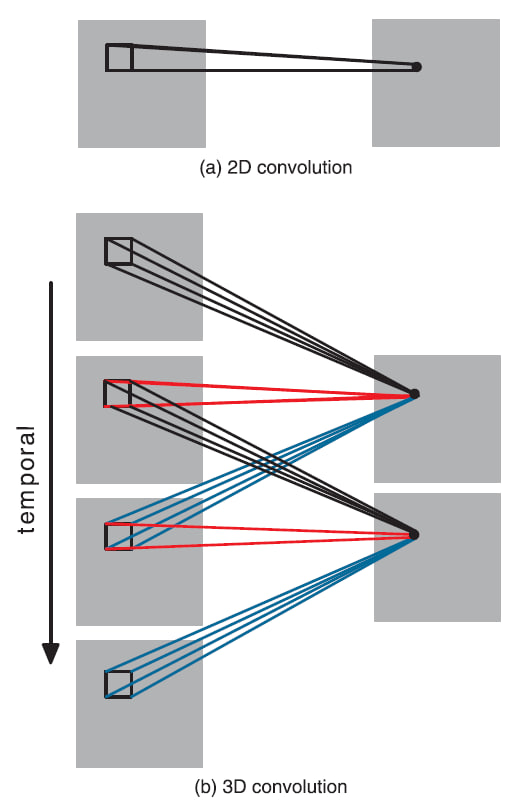
\includegraphics[width=0.8\textwidth]{archivos/figuras/comparison.jpg} 
    \caption{A visual comparison of (a) 2D convolution and (b) 3D convolution.}
    \label{fig:2d_vs_3d}
\end{figure}

\subsection{Learning Multiple Feature Types}
A single 3D kernel, when applied across the video cube, can only extract one type of spatio-temporal feature. To build a rich and discriminative representation, a 3D CNN layer applies multiple, distinct 3D kernels in parallel to the same input volume. Each kernel learns to respond to a different kind of motion or appearance pattern. This results in the creation of multiple feature map "channels" at the output of the layer, where each channel represents a different aspect of the learned action.

\begin{figure}[H]
    \centering
    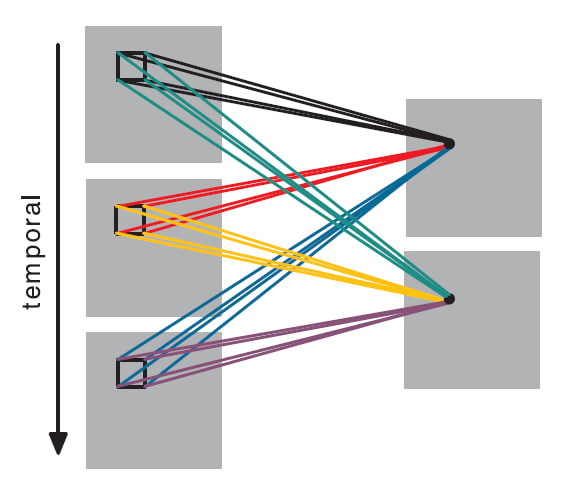
\includegraphics[width=0.8\textwidth]{archivos/figuras/extraction.jpg} 
    \caption{Extraction of multiple features using multiple distinct 3D convolution kernels.}
    \label{fig:multiple_features}
\end{figure}

\subsection{A 3D CNN Architecture for Action Recognition}

Based on the 3D convolution operation, the paper proposes a complete, end-to-end deep learning architecture for human action recognition. The model, shown in Figure \ref{fig:3d_arch}, consists of a series of alternating 3D convolutional and subsampling (pooling) layers.

The network takes a short clip of video (e.g., 7 contiguous frames) as input. The initial layers perform pre-processing by computing gradients and optical flow to create multiple input channels. This is followed by a stack of learnable layers:
\begin{enumerate}
    \item \textbf{3D Convolutional Layers (C2, C4):} These layers apply banks of 3D kernels to learn spatio-temporal features, as described above.
    \item \textbf{Subsampling Layers (S3, S5):} After each convolution, a pooling operation (e.g., max pooling) is applied to reduce the spatial resolution of the feature maps. This provides a degree of translation invariance and aggregates the learned features over larger regions.
    \item \textbf{Fully Connected Layer (C6):} After several stages of feature extraction, the final feature maps are flattened into a single 128-dimensional feature vector. This vector is a compact, high-level representation of the action that occurred in the input clip.
    \item \textbf{Output Layer:} This final feature vector is fed into a classifier (e.g., a softmax layer) that makes the final prediction about which action class the video belongs to.
\end{enumerate}
This architecture demonstrates how to construct a deep, hierarchical model that learns progressively more complex and abstract representations of motion directly from pixels.

\begin{figure}[H]
    \centering
    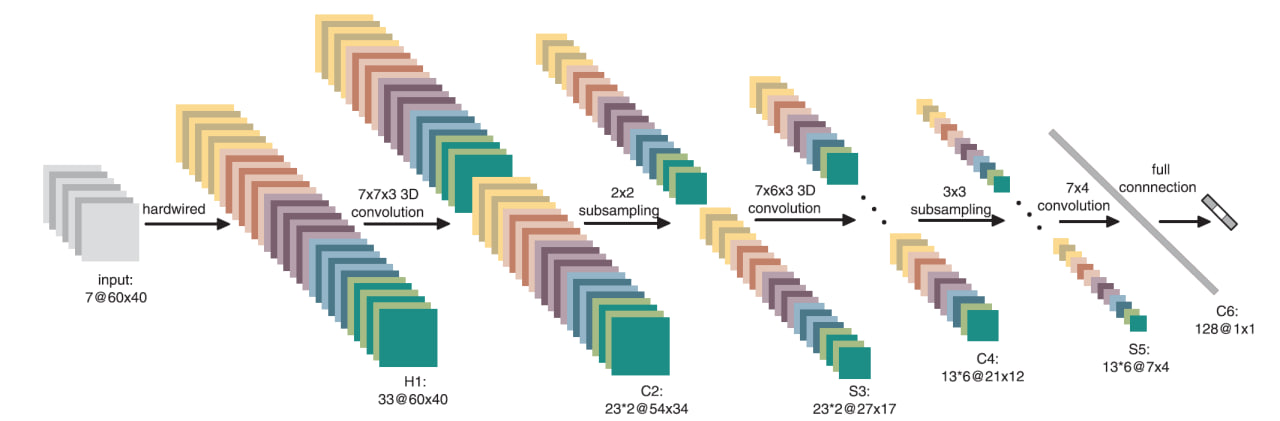
\includegraphics[width=0.8\textwidth]{archivos/figuras/architecture.jpg} 
    \caption{A complete 3D CNN architecture for human action recognition.}
    \label{fig:3d_arch}
\end{figure}

\subsection{Implications for Video Analysis}

The introduction of 3D CNNs represents a significant milestone in video understanding. It provides a principled and effective way to build end-to-end models that learn spatio-temporal features in a unified manner. Unlike hybrid CNN-RNN models that treat space and time separately, 3D CNNs fuse these dimensions at the earliest stages of processing. This approach has proven to be highly effective and has become a foundational technique in the field of video-based action recognition, directly influencing many subsequent state-of-the-art models. The principles developed for recognizing human actions are directly transferable to other domains, including the automated analysis of animal or bird behavior from video.

\section{SimBA: Simple Behavioral Analysis Toolkit}

Simple Behavioral Analysis (SimBA) is an open-source toolkit designed for the automated classification of complex social behaviors in experimental animals using video data. Although originally developed for rodents, the principles underlying SimBA — such as pose estimation–based feature extraction and supervised behavior classification — are highly transferable to other species. In the context of bird behavior analysis, similar pipelines can be employed to detect and classify movement patterns, especially when combined with pose-tracking tools and machine learning models. SimBA highlights the growing importance of accessible, reproducible workflows for video-based behavioral studies, which directly aligns with the goals of this work.

\subsection{The Challenge and Limitations of Manual Behavioral Annotation}

The study of animal behavior, particularly complex social interactions, is fundamental to neuroscience and psychology. However, the traditional method for quantifying these behaviors—manual annotation by a trained human observer—presents significant bottlenecks. This process is:
\begin{itemize}
    \item \textbf{Time-Intensive:} Manually scoring hours of video is an arduous and slow process, limiting the scale of experiments.
    \item \textbf{Subjective:} The definition of a behavior can vary between observers, leading to poor inter-rater reliability. It is also susceptible to "observer drift," where an individual's scoring criteria may subtly change over time.
    \item \textbf{Low-Resolution:} Manual annotation cannot capture the millisecond-scale dynamics of behavior, making it difficult to correlate with fast neural recording techniques like fiber photometry or electrophysiology.
\end{itemize}
To overcome these challenges, the field has increasingly turned to machine learning. The SimBA toolkit presented in this paper exemplifies a modern, powerful, and accessible pipeline for automating this process.

\subsection{The Paradigm Shift: From Pixels to Pose}

Instead of attempting to classify actions directly from raw video pixels, the SimBA workflow is built on a more structured, two-stage approach. The first and most critical step is to use a deep convolutional neural network not for action classification, but for \textbf{pose-estimation}.

\subsection{Pose-Estimation with Deep Learning}
Tools like \textbf{DeepLabCut} and \textbf{DeepPoseKit} are used to track the (x, y) coordinates of a set of user-defined body parts on each animal in every frame of the video. The user first manually labels a few hundred frames to train the network. Once trained, the pose-estimation model can automatically predict the location of these body parts (e.g., nose, ears, paws, tail-base) with high accuracy, even in cluttered environments. This crucial first step transforms the unstructured problem of video analysis into a highly structured time-series problem: the output is no longer a video, but a set of coordinate data representing the dynamic posture of the animals over time.

\begin{figure}[H]
    \centering
    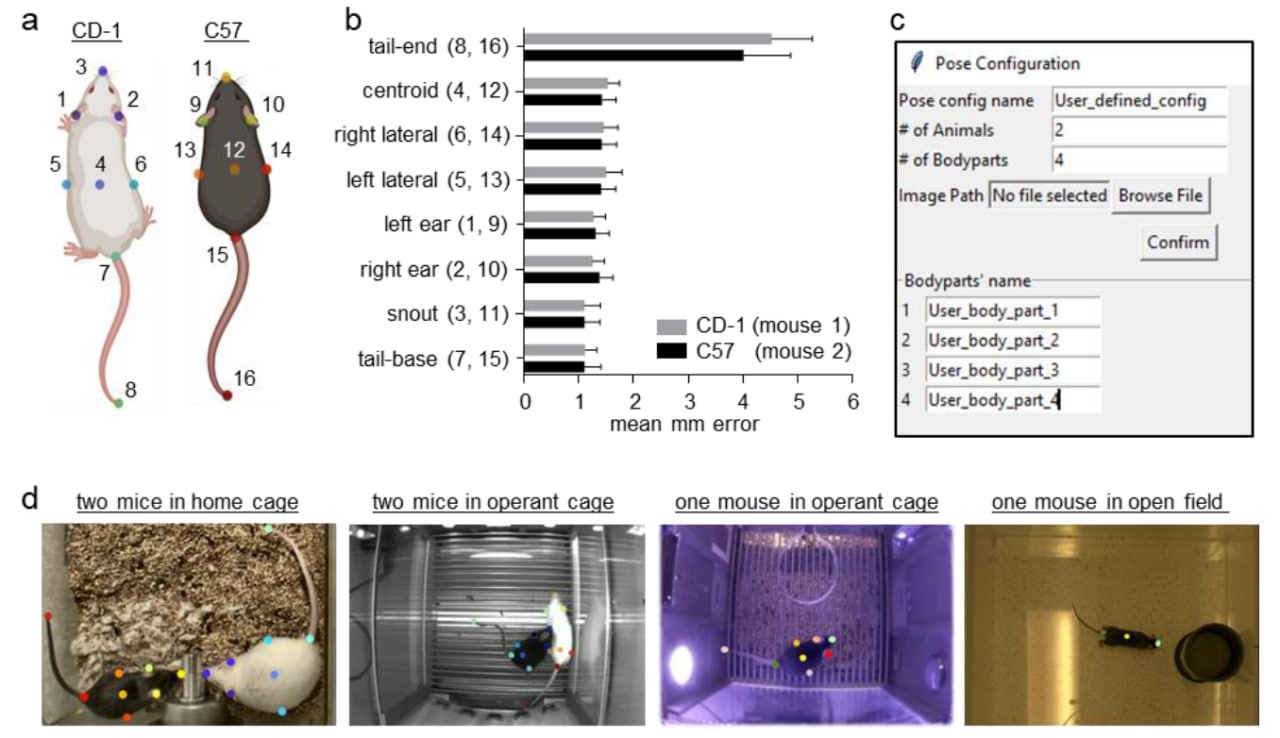
\includegraphics[width=0.8\textwidth]{archivos/figuras/animal_tracking.jpg} 
    \caption{Animal pose-estimation body-part tracking. (a) A schematic of 16 body parts tracked on two mice. (c) The flexible interface in SimBA for defining custom tracking schemas. (d) Examples of different tracking schemas. This figure is fundamental to understanding that the initial data for behavior classification is the animal's skeleton, not the raw image.}
    \label{fig:pose_estimation}
\end{figure}

\subsection{From Pose Data to Behavioral Features}

With the time-series of body-part coordinates, the next step is \textbf{feature engineering}. The SimBA toolkit automatically calculates a large and comprehensive set of features from this raw tracking data. These are not learned features in the traditional deep learning sense, but are mathematically derived metrics that capture the geometry and dynamics of the animals' interactions. Examples of such features include:

\begin{itemize}
    \item The distance between the nose of animal 1 and the tail-base of animal 2.
    \item The velocity and acceleration of each individual body part.
    \item The angle between three body parts (e.g., nose, centroid, tail-base) to measure posture.
    \item The area of the convex hull enclosing all of an animal's body parts.
    \item The movement of body parts relative to each other.
\end{itemize}
By calculating hundreds of such features for each frame, the system creates a rich, high-dimensional representation of the animals' behavior that is primed for machine learning.

\subsection{Supervised Classification of Behaviors}

The final step in the pipeline is to use a supervised machine learning model to classify behaviors based on the engineered feature set. The paper uses \textbf{Random Forest classifiers}, which are an ensemble of decision trees.

The workflow is as follows:
\begin{enumerate}
    \item \textbf{Annotation:} A human expert uses a simple event logger in SimBA to label short segments of the video with the behavior of interest (e.g., "attack", "pursuit", "sniffing"). This provides the ground-truth data.
    \item \textbf{Training:} The Random Forest model is trained on the feature data from the annotated frames. It learns to find the statistical patterns in the feature space that correspond to the expert's behavioral labels. For example, it might learn that an "attack" is characterized by a low nose-to-nose distance, high velocity of the attacking animal's centroid, and a specific postural angle.
    \item \textbf{Prediction:} Once trained, the classifier can be applied to new, unlabeled videos to automatically predict the presence or absence of the target behavior on a frame-by-frame basis, achieving millisecond resolution.
\end{enumerate}

\subsection{The SimBA Workflow: Ensuring Accessibility and Transparency}
A core contribution of the SimBA paper is not just the methodology, but the creation of an accessible, open-source toolkit with a Graphical User Interface (GUI). This allows researchers without extensive programming knowledge to implement this entire pipeline. The workflow is explicitly designed with validation and explainability in mind.

\begin{figure}[H]
    \centering
    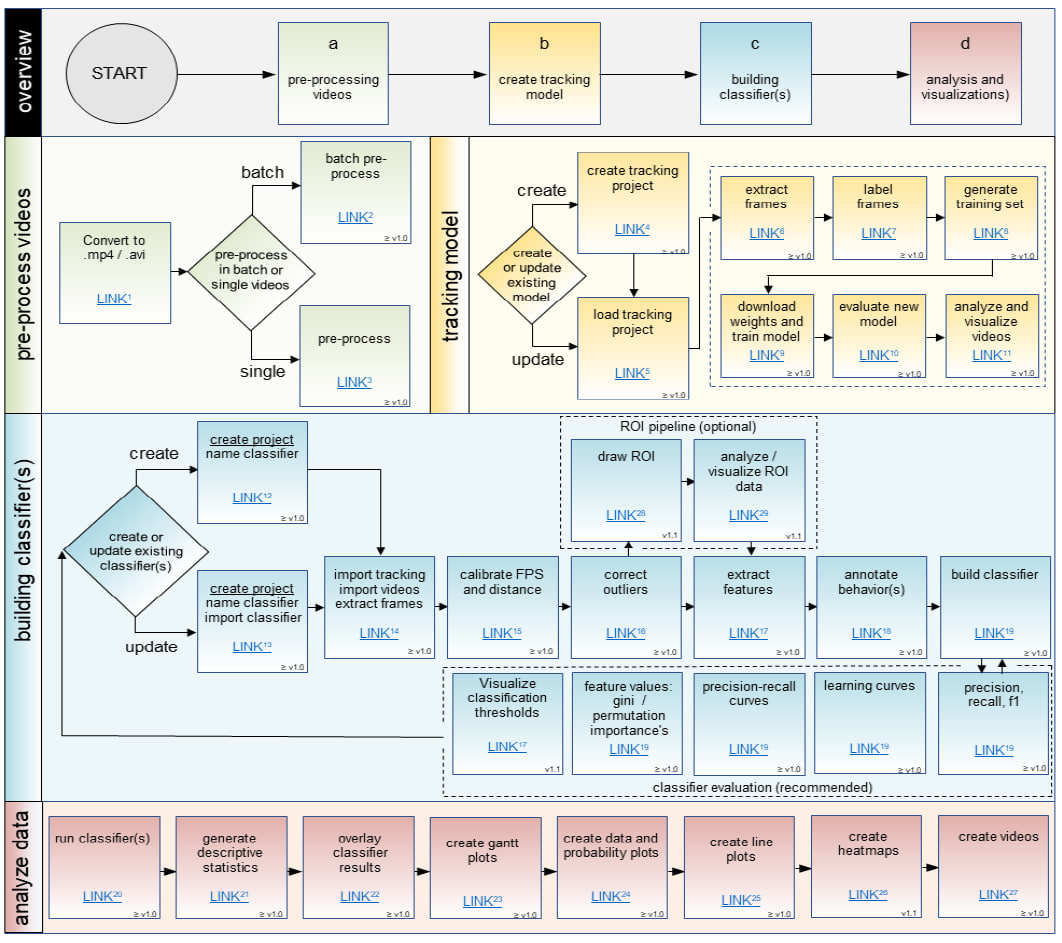
\includegraphics[width=0.8\textwidth]{archivos/figuras/flowchart_simba.jpg} 
    \caption{The complete SimBA workflow for creating supervised machine learning classifiers.}
    \label{fig:simba_workflow}
\end{figure}

To combat the "black-box" nature of some machine learning models, SimBA includes tools to interpret the classifier's decisions. One of the most important tools is the calculation of \textbf{feature permutation importance}. This technique measures how much the classifier's accuracy drops when the values of a single feature are randomly shuffled. Features that cause a large drop in performance are considered highly important for the model's predictions. This allows the researcher to verify that the model is using biologically relevant cues to classify behavior.

\begin{figure}[H]
    \centering
    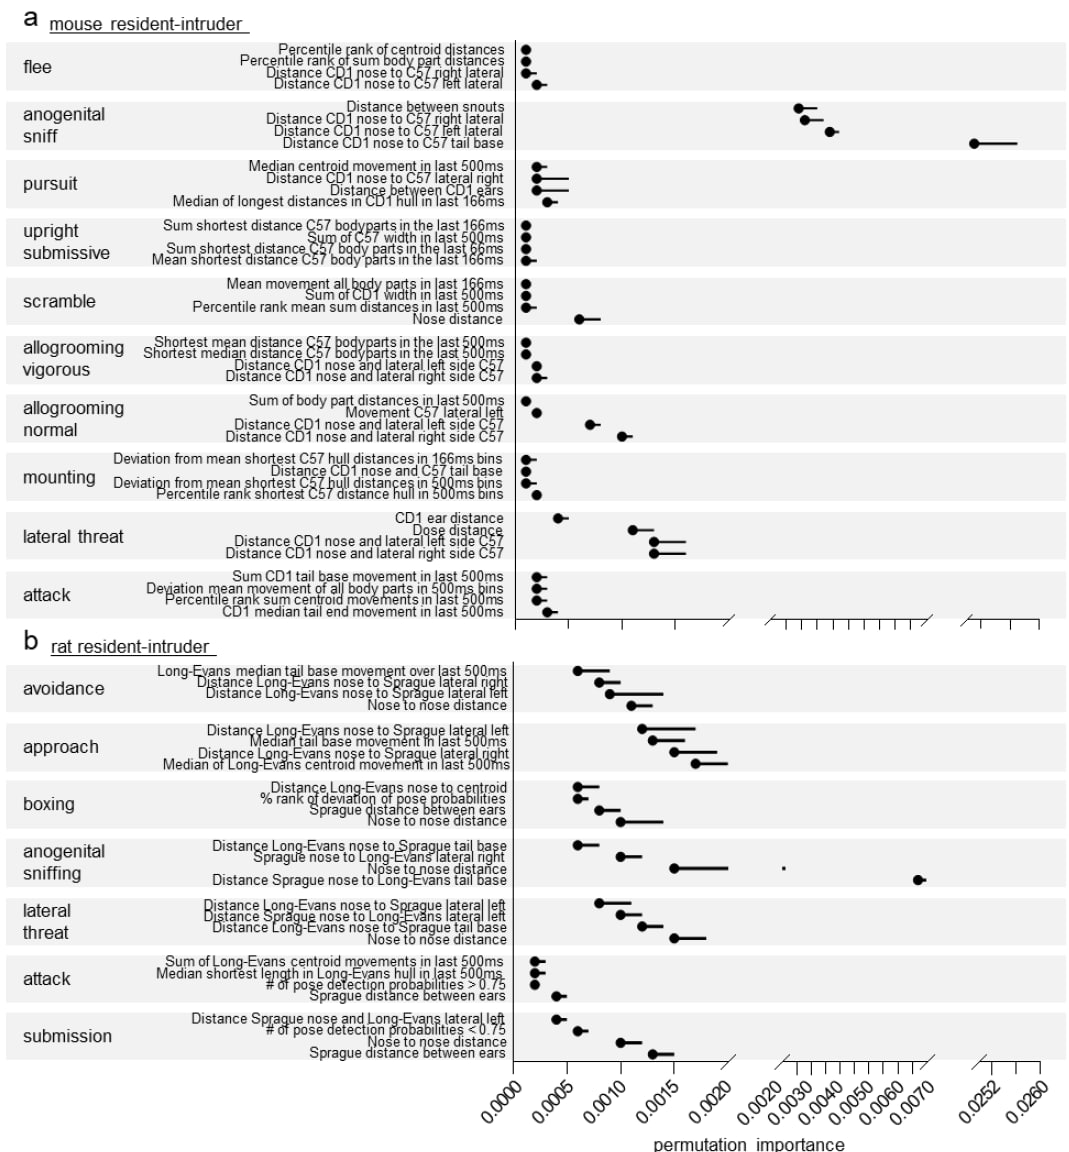
\includegraphics[width=0.8\textwidth]{archivos/figuras/permutation.jpg} 
    \caption{Feature permutation importances for classifiers.}
    \label{fig:feature_importance}
\end{figure}

This comprehensive, pose-estimation-based workflow represents the current state-of-the-art for detailed, objective, and high-throughput analysis of complex behaviors in experimental animals, and its principles can be readily adapted for the study of other species.

\section{PyRat: open-source Python library}

PyRAT is an open-source Python library developed for the analysis of animal behavior using pose estimation data. It provides a modular framework for processing, visualizing, and classifying behavioral sequences based on body keypoints over time. While PyRAT has primarily been applied to small mammals, its core methodology — including trajectory analysis, feature extraction, and machine learning–based behavior classification — can be readily adapted to bird species. In this project, similar strategies are employed to analyze and interpret fine-grained avian motion patterns, underscoring the broader applicability of pose-based behavioral analysis tools.

\subsection{An Alternative to Supervised Classification}

While supervised machine learning, as exemplified by toolkits like SimBA, provides a powerful means to automate the classification of pre-defined behaviors, it is fundamentally dependent on extensive manual annotation. This process requires a human expert to provide the ground-truth labels that the model learns to replicate. As the paper by De Almeida et al. (2022) implicitly suggests, an alternative and complementary approach is \textbf{unsupervised learning}. This paradigm aims to identify and cluster distinct animal behaviors automatically, without the need for a priori labels. The Python Rodent Analysis and Tracking (PyRAT) library is presented as a toolkit for implementing such an unsupervised workflow.

The core philosophy is to let the structure of the data itself reveal the underlying behavioral repertoire of the animal. This is particularly useful for exploratory analysis, where the goal is to discover novel behavioral patterns rather than simply quantifying known ones.

\subsection{The PyRAT Pipeline: From Pose to Unsupervised Clustering}

Similar to other modern frameworks, the PyRAT pipeline begins by converting raw video data into a structured format using deep learning-based pose-estimation. However, it diverges significantly in how it processes this structured data.

\subsection{Pose-Estimation as a Foundational Input}
The workflow starts with coordinate data from a pose-estimation tool like DeepLabCut. This provides a time-series of the (x, y) locations for a set of defined body parts. This initial step is identical to the supervised pipeline and serves to represent the animal's continuous posture and movement as a structured dataset.

\begin{figure}[H]
    \centering
    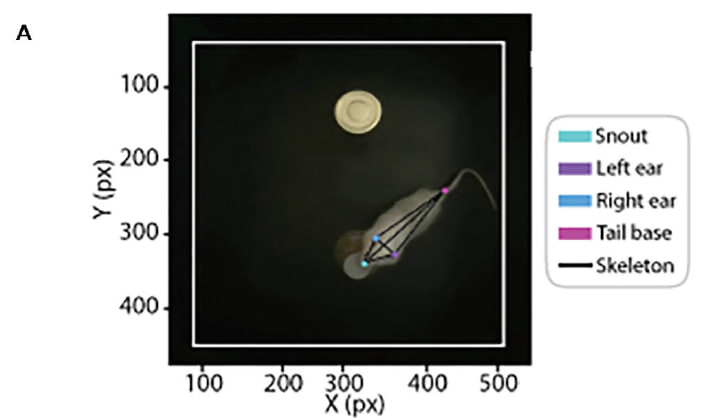
\includegraphics[width=0.8\textwidth]{archivos/figuras/pyrat_1a.jpg} 
    \caption{The foundational input for the PyRAT library: pose-estimation data.}
    \label{fig:pose_input}
\end{figure}

\subsection{Unsupervised Behavior Classification}
Instead of training a model on human labels, PyRAT's core function, \texttt{ClassifyBehavior()}, performs an unsupervised analysis. The process is two-fold:

\begin{enumerate}
    \item \textbf{Hierarchical Agglomerative Clustering:} The primary input for the algorithm is the set of pairwise distances between all tracked body parts for each frame. This feature representation is inherently invariant to the animal's position and orientation in the arena. The algorithm then groups frames with similar postural configurations (i.e., similar inter-body-part distances) together. This results in the automatic generation of distinct behavioral clusters. For example, postures corresponding to "rearing" will have a large distance between the nose and tail-base and will be grouped into one cluster, while "grooming" postures will have a small nose-to-paw distance and will form another.

    \item \textbf{t-SNE for Visualization:} To help researchers visualize and interpret these high-dimensional clusters, PyRAT uses t-distributed Stochastic Neighbor Embedding (t-SNE). This is a non-linear dimensionality reduction technique that projects the complex feature data into a 2D space while preserving local neighborhood structure. The result is a map where each point represents a single frame of video, and frames belonging to the same behavioral cluster appear grouped together. The researcher can then inspect the video segments corresponding to each cluster to assign a meaningful ethological label (e.g., "rearing," "locomotion," "immobility").
\end{enumerate}

\begin{figure}[H]
    \centering
    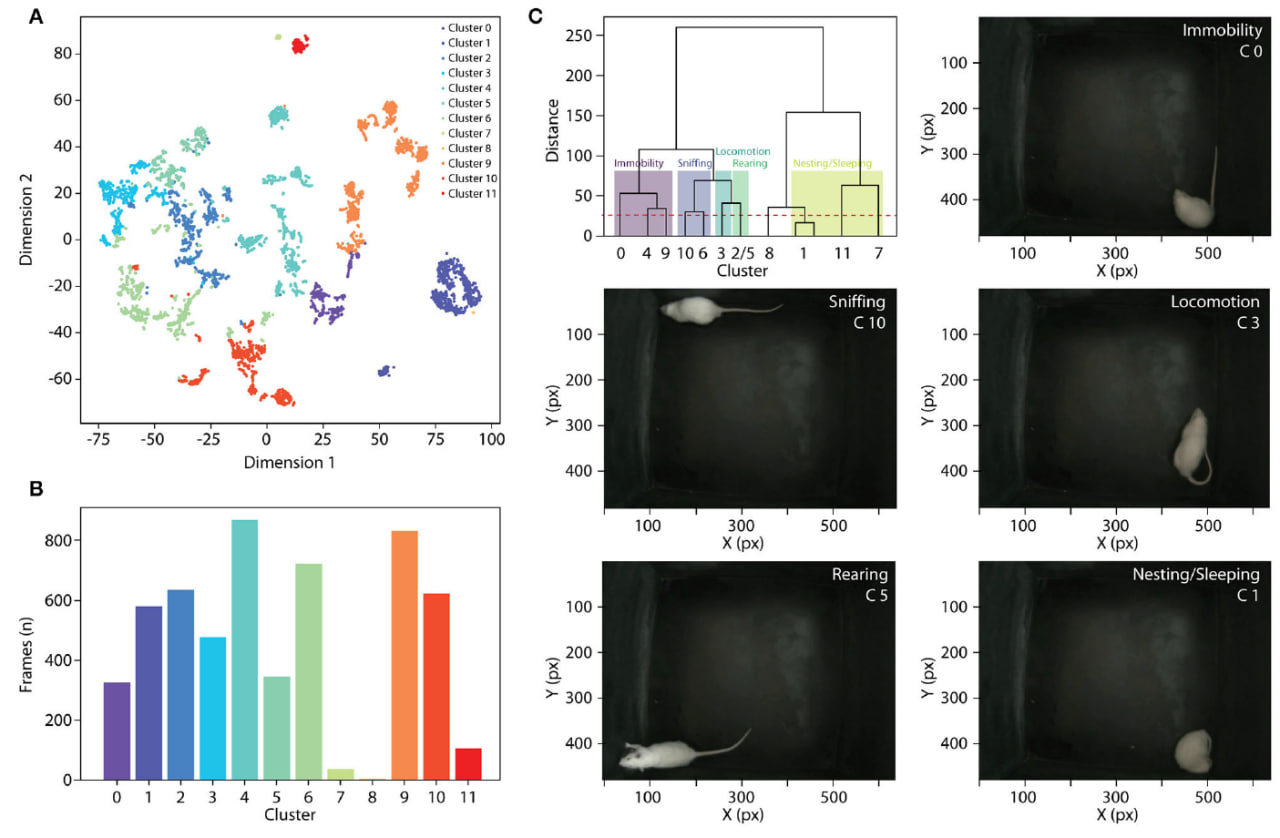
\includegraphics[width=0.8\textwidth]{archivos/figuras/pyrat_3.jpg} 
    \caption{The unsupervised behavior classification process in PyRAT. (A) A t-SNE plot visualizing the automatically discovered clusters. (B) A histogram showing the number of frames in each cluster. (C) A dendrogram from the hierarchical clustering, with example frames from the five identified behavioral classes. This figure provides a complete overview of the unsupervised discovery workflow.}
    \label{fig:unsupervised_clustering}
\end{figure}

\subsection{Kinematic Analysis and Integration with Neural Data}

Beyond behavioral clustering, PyRAT provides a suite of tools for quantifying standard locomotor and kinematic metrics from the pose-estimation data. These functions allow for the analysis of:
\begin{itemize}
    \item \textbf{Trajectory and Occupancy:} Visualizing where the animal has been and how much time it has spent in different parts of the arena using trajectory plots and heatmaps.
    \item \textbf{Motion Metrics:} Calculating instantaneous speed, acceleration, and total distance traveled.
    \item \textbf{Object Interaction:} Quantifying the time spent interacting with specific user-defined regions or objects.
\end{itemize}

\begin{figure}[H]
    \centering
    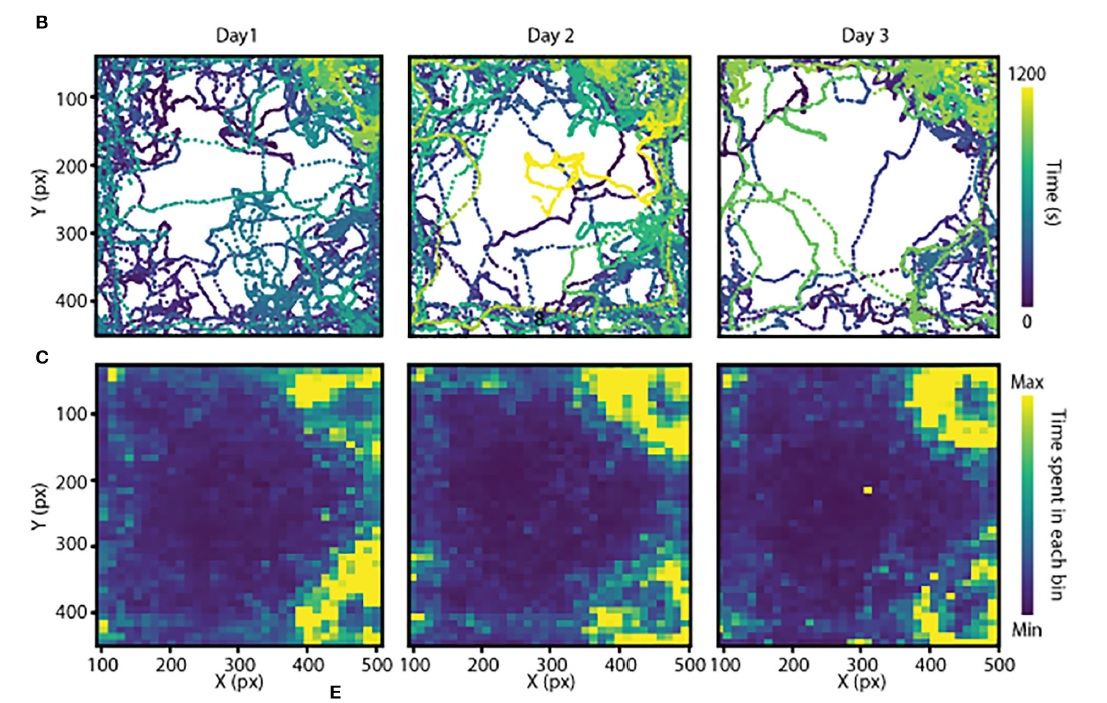
\includegraphics[width=\textwidth]{archivos/figuras/pyrat_1bc.jpg} 
    \caption{Kinematic analysis in PyRAT. (B) Trajectory plots showing the path of a rat over three consecutive days, with color indicating time. (C) Occupancy heatmaps showing the average time spent in each location. These are standard, essential analyses for behavioral studies.}
    \label{fig:kinematics}
\end{figure}

A key strength of the library is its built-in functionality for integrating these behavioral analyses with synchronized neural data. PyRAT includes functions that can take the timestamps of the automatically discovered behavioral clusters and use them to extract corresponding epochs from electrophysiology recordings (e.g., raw LFP or spike train data). This enables researchers to directly investigate the neural correlates of spontaneously expressed behaviors.

\begin{figure}[H]
    \centering
    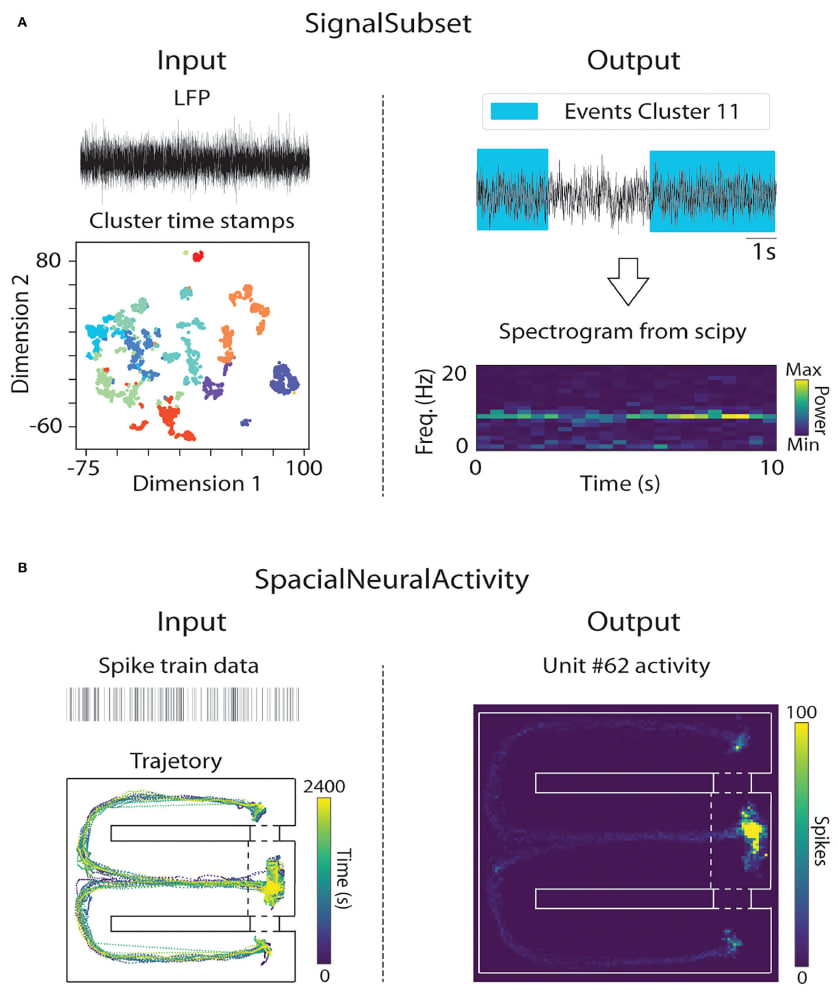
\includegraphics[width=0.8\textwidth]{archivos/figuras/pyrat_4.jpg} 
    \caption{Integration of behavioral and neural data. (A) The \texttt{SignalSubset} function uses the timestamps from a behavioral cluster to extract corresponding segments of LFP data. (B) The \texttt{SpacialNeuralActivity} function creates a heatmap of neural firing rate as a function of the animal's position in the arena. (Based on Figure 4 from De Almeida et al., 2022).}
    \label{fig:neural_integration}
\end{figure}

\subsection{Supervised vs. Unsupervised Approaches: A Complementary View}
The PyRAT paper highlights a different philosophy from the supervised approach of SimBA.
\begin{itemize}
    \item \textbf{Supervised methods} are ideal for \textit{hypothesis testing}. A researcher defines a specific behavior of interest, and the model quantifies its occurrence with high accuracy.
    \item \textbf{Unsupervised methods} are ideal for \textit{hypothesis generation}. The model discovers all the distinct behavioral patterns present in the data, potentially revealing novel or subtle behaviors that a human observer might miss.
\end{itemize}
Together, these two paradigms represent a powerful and comprehensive toolkit for modern computational neuroethology, allowing for both the precise measurement of known behaviors and the unbiased discovery of new ones.

\section{3D-POP - An automated annotation approach for bird behavior}

The 3D-POP framework presents an automated annotation method that bridges marker-based motion capture and markerless tracking for freely moving birds. While it focuses on 3D pose recovery from motion capture data, its core contribution — aligning 2D keypoints with accurate 3D ground truth — is highly relevant for training and validating computer vision models in animal behavior analysis. In this work, we build on similar principles by leveraging pose-based representations to classify and interpret bird behaviors from video. Tools like 3D-POP help establish high-quality training data, enabling more precise and biologically meaningful behavior recognition in markerless settings.

\subsection{The Data Bottleneck in Animal Pose-Estimation}

The success of any data-driven, deep learning model is critically dependent on the quality and quantity of its training data. In the field of animal behavior analysis, this presents a formidable challenge. As highlighted in the work by Naik et al. (2022), while markerless pose-estimation tools have revolutionized the field, they are fundamentally limited by the availability of large, accurately annotated datasets.

Manual annotation of video frames is the most common method for generating training data, but it is plagued by several issues:
\begin{itemize}
    \item \textbf{Labor-Intensive:} The process is extraordinarily slow, making the creation of datasets with millions of labeled instances impractical.
    \item \textbf{Inaccurate:} It is difficult for human annotators to consistently and precisely locate keypoints, especially in low-resolution video or during fast movements.
    \item \textbf{Lack of 3D Ground Truth:} Manual annotation is inherently a 2D process. Generating accurate 3D ground-truth data for animals in motion is nearly impossible through manual labeling alone. This severely hampers the development of models that aim to reconstruct an animal's full 3D posture, which is essential for a complete biomechanical understanding of behavior.
\end{itemize}
The 3D-POP paper directly confronts this "data bottleneck" by proposing a novel, semi-automated method for generating a massive, high-precision 2D and 3D dataset for freely moving birds.

\subsection{A Novel Solution: Semi-Automated Annotation via Motion Capture}

The core innovation of the 3D-POP project is the use of a professional \textbf{motion capture (mo-cap) system} as a tool for generating ground-truth data for training markerless tracking systems. This hybrid approach leverages the strengths of two different technologies to create a "best of both worlds" data generation pipeline.

\subsection{The Hybrid Mo-Cap and Video Setup}
The experimental setup involves a large arena monitored simultaneously by:
\begin{enumerate}
    \item A multi-camera, high-speed \textbf{motion capture system} (e.g., Vicon) that tracks the sub-millimeter 3D position of small, reflective markers.
    \item Several high-resolution \textbf{RGB video cameras} that record the scene from different viewpoints.
\end{enumerate}
Birds in the experiment are fitted with a small, lightweight backpack and head-mounted base, onto which the reflective mo-cap markers are attached. The mo-cap system provides highly accurate 6-DOF (Degrees of Freedom) tracking of the head and body segments, while the RGB cameras capture the natural appearance of the birds.

\begin{figure}[H]
    \centering
    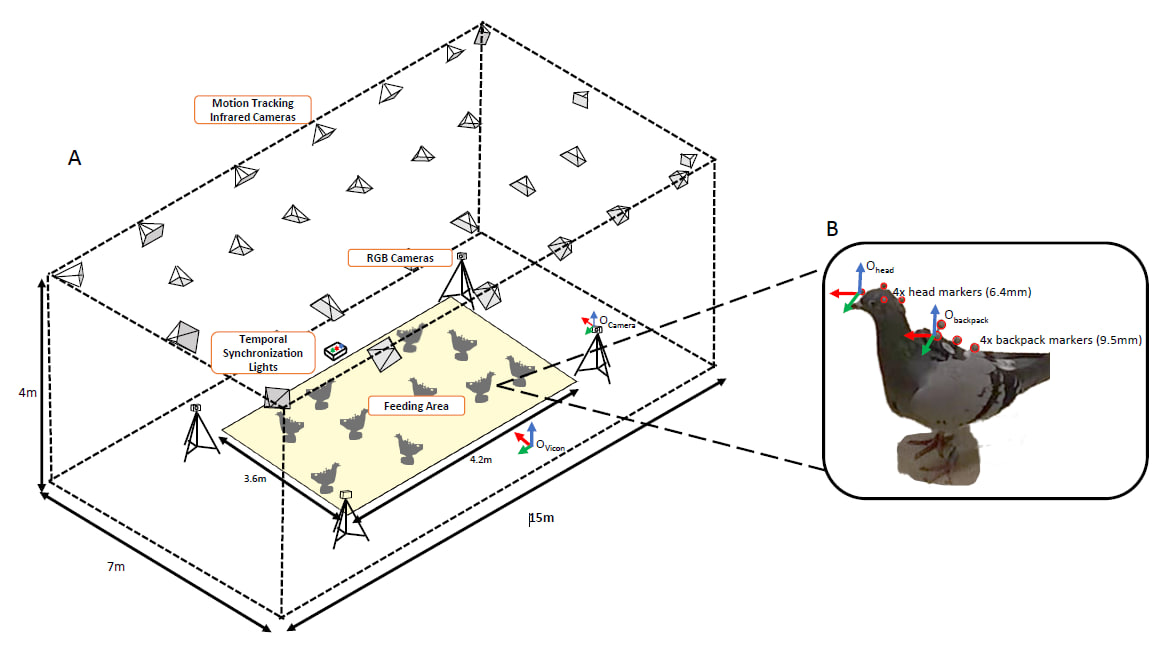
\includegraphics[width=0.8\textwidth]{archivos/figuras/setup1.jpg} 
    \caption{The experimental setup for the 3D-POP dataset. (A) The layout of the arena with motion tracking infrared cameras and synchronized RGB cameras. (B) A pigeon subject with reflective markers attached to a head mount and a backpack. This hybrid setup is the key to the semi-automated annotation method. (Based on Figure 2 from Naik et al., 2022).}
    \label{fig:setup}
\end{figure}

\subsection{The Annotation Principle: From Markers to Morphological Keypoints}
A key challenge is that it is often impossible to place a physical marker directly on the morphological keypoint of interest (e.g., the tip of the beak or the center of the eye). The 3D-POP method cleverly overcomes this by establishing a rigid spatial relationship between the tracked markers and the desired keypoints.

The process is as follows:
\begin{enumerate}
    \item For each bird, a human annotator manually labels the desired morphological keypoints (beak, eyes, tail, etc.) in a small number of frames (5-10) from multiple camera views.
    \item The system then computes the fixed 3D position of these keypoints \textit{relative} to the coordinate system of the tracked markers on the head and backpack. This creates a "digital skeleton" for the bird.
    \item By assuming the head and body are largely rigid bodies, this relationship remains constant.
\end{enumerate}

\subsection{From Manual Annotation to Automated Propagation}
Once this rigid relationship is established, it can be used to automatically generate annotations for the entire video dataset. For any given frame, the mo-cap system provides the precise 3D position and orientation of the markers. The system can then use the pre-computed "digital skeleton" to calculate the corresponding 3D position of all the morphological keypoints. These 3D points are then projected back into the 2D image plane of each RGB camera to generate highly accurate 2D keypoint labels. This allows for the creation of millions of accurately labeled instances with only a few minutes of manual annotation effort per subject.

\begin{figure}[H]
    \centering
    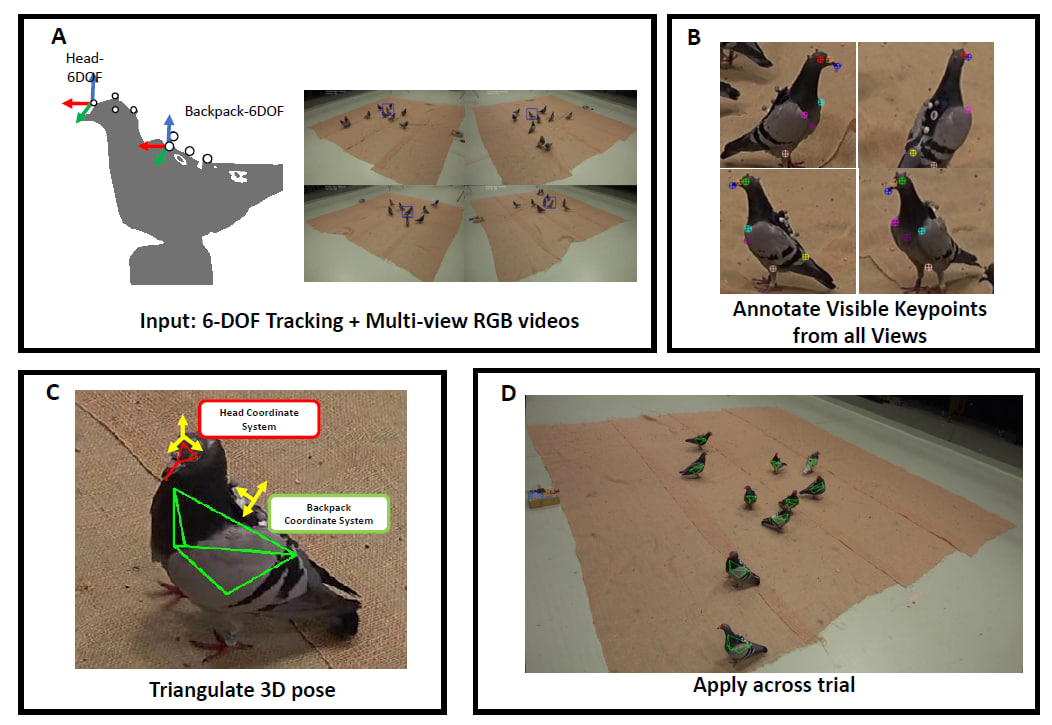
\includegraphics[width=0.8\textwidth]{archivos/figuras/setup2.jpg} 
    \caption{The semi-automated annotation pipeline. (A) The system takes the 6-DOF tracking data and multi-view videos as input. (B) A user manually annotates keypoints in a few frames. (C) The system triangulates the 3D positions of the keypoints relative to the markers. (D) This relationship is then propagated across all frames of all trials to generate the full dataset.}
    \label{fig:pipeline}
\end{figure}

\subsection{The 3D-POP Dataset and Its Implications}

The result of this pipeline is the \textbf{3D-POP (3D Postures of Pigeons) dataset}, the first large-scale dataset of flocking birds featuring accurate ground truth for 2D keypoints, 3D keypoints, bounding boxes, and individual identities across multiple individuals and camera views.

The significance of this contribution is twofold:
\begin{enumerate}
    \item \textbf{Enabling Robust Markerless Models:} This dataset provides the necessary training data to develop and validate powerful, deep learning-based models for markerless 2D and 3D pose-estimation in birds. As the authors demonstrate, a model trained on this data can accurately track the posture of birds that have no markers attached.
    \item \textbf{Facilitating 3D Behavioral Analysis:} By providing accurate 3D ground truth, the dataset opens the door to research that moves beyond 2D analysis. It enables the development of models that can reconstruct a bird's full 3D posture from 2D video, a critical step for biomechanical and advanced behavioral studies.
\end{enumerate}

\begin{figure}[H]
    \centering
    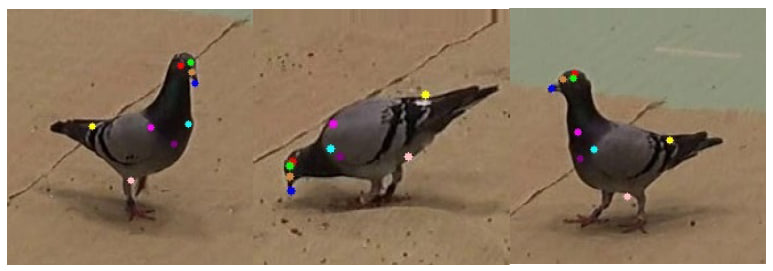
\includegraphics[width=0.8\textwidth]{archivos/figuras/pigeons.jpg} 
    \caption{Proof of concept for markerless tracking.}
    \label{fig:markerless_prediction}
\end{figure}

It establishes that the quality of the underlying training data is paramount and presents a state-of-the-art methodology for generating it. While this thesis may not construct a new dataset of this scale, it will leverage models and techniques that are trained on such high-quality data, and the principles of moving from 2D tracking towards 3D understanding remain a guiding ambition for the field.


\section{Summary}

In aggregate, the reviewed literature provides a clear and comprehensive roadmap for the state-of-the-art in automated animal behavior analysis. The central, unifying conclusion is the paradigm shift away from end-to-end action recognition towards a more robust and interpretable two-stage pipeline. This modern workflow, exemplified by frameworks like SimBA, first leverages powerful deep convolutional neural networks (such as DeepLabCut) for markerless pose-estimation. This critical initial step transforms unstructured video data into a structured time-series of kinematic coordinates. Subsequently, a supervised machine learning classifier, typically a Random Forest, is trained on a rich set of engineered features derived from these coordinates—such as velocities, angles, and distances—to classify pre-defined behaviors with high temporal precision and accuracy. The work on the 3D-POP dataset underscores that the success of this entire pipeline is fundamentally dependent on the creation of a large-scale, high-quality annotated dataset for training the initial pose-estimation model, establishing data generation as a critical scientific contribution in its own right.

For this master's thesis, these articles provide both the strategic justification and the technical foundation for the proposed methodology. The foundational papers on 3D CNNs and Hybrid Vision Transformers (HVTs) justify the selection of deep learning architectures as the optimal tools for extracting rich spatio-temporal features from video. The more recent papers on the SimBA, PyRAT, and 3D-POP workflows provide the practical blueprint for the project's design: first, to dedicate significant effort to creating an accurately annotated dataset of bird keypoints to train a robust pose-estimation model; and second, to build a classification system upon the resulting kinematic data. By integrating these insights, this project is not merely applying a set of disconnected techniques but is implementing a cohesive, state-of-the-art methodology that is validated by the scientific community, ensuring that its contributions are both technologically sound and ecologically relevant.